\section{Analysis of forward neutrons \label{sec-ananc}}
\subsection{Analysis method}
A momentum of a forward neutral particle is measured by the time-of-flight method between T0 and the NC. % as schematically illustrated in Fig. \ref{fig-ncconcept}. 
The velocity of the forward particle can be expressed as,
\begin{eqnarray}
\beta_{nc} &=& \frac{L_{vertex-NC} }{(T^{measured}_{T0-NC}-T^{calc}_{T0-vertex})\times c} \label{eq-ncbeta}
\end{eqnarray}
where, $L_{vertex-NC}$ is the flight length between the hit position on the NC and the reaction vertex obtained by the BPC and the CDC as described in Sec. 3.4.3, $T^{measured}_{T0-NC}$ is the measured flight time between T0 and the NC, and $T^{calc}_{T0-vertex}$ is the calculated time between T0 and the vertex by using reconstructed beam momentum. The hit position on T0 was obtained from an extrapolation of the BLC2 track, and the momentum decrease of the kaon beam due to the energy losses in the spectrometer materials were considered.

%Note that the current analysis method always requires at least one CDC track and unavoidably make bias in the final spectrum.

\subsection{NC hit selection}
To obtain the flight time of the neutral particle and its hit position on the NC, we selected the time-wise first-hit segment of the NC whose energy deposit was above the offline analysis threshold. The hit positions in the $x$- and $z$-directions were defined as the center of the segment, and that in $y-$direction was evaluated from the time difference of the two PMT signals on both ends of the segment. To convert from the time difference to the $y$ position, we used the effective light propagation velocity of 14 cm/ns, which was measured with a $^{90}$Sr checking source.

\subsection{Charge removal}
There were two scintillation counter arrays, the BVC and the CVC, between the target and the NC. To assure neutral-particle detection with the NC, no signal in the BVC and the CVC was required. The time range of the TDCs for those counters were set to 200 ns, whose full range was used for the simplicity to veto forward-going charged particles. The over veto efficiency is evaluated in Sec. \ref{sec-overveto}.

\subsection{1/$\beta$ distribution}
Figure \ref{fig-ncbeta} shows $1/\beta$ distribution of the neutral particles without offline threshold of the energy deposit on the NC. Hardware-wise, we set the threshold of discriminators to around 0.5 MeV$ee$. The distribution shows a distinct $\gamma$-ray peak at $1/\beta=1$, with which we calibrated the relative time offset of the NC counters and the T0 counters. In the slower velocity region, namely the larger $1/\beta$ region, continuous distribution of neutrons can be seen. The TDCs used for the NC had 200 ns time ranges and we adjusted the start timing to detect the particles with ($-$25, 175) ns offset to the gamma-ray TOF. It corresponds to down to 200 MeV/$c$ neutrons. A peak structure around $1/\beta=1.3$ is the so-called quasi-free peak attributed to the reactions of $``p"(K^-,n)K^0_s$ and $``n"(K^-,n)K^-$. Our interested region is between the $\gamma$-ray peak and the quasi-free peak, where a clear gap is observed. This shows the low background condition in our measurement. The accidental background yield can be directly evaluated with the strength of the left part of the $\gamma$-ray peak.

\subsubsection{Particle identification}
The neutral particles with $1/\beta>1.1$ were identified as neutrons, whereas gate for $\gamma$-rays were defined to be (0.9,1.1). Then, we can obtain the neutron momentum $p_n$ with the neutron mass $m_n$,
\begin{eqnarray}
p_n &=& \frac{m_n}{\sqrt{\frac{1}{\beta^2}-1}}.
\end{eqnarray}

\begin{figure}[]
\begin{center}
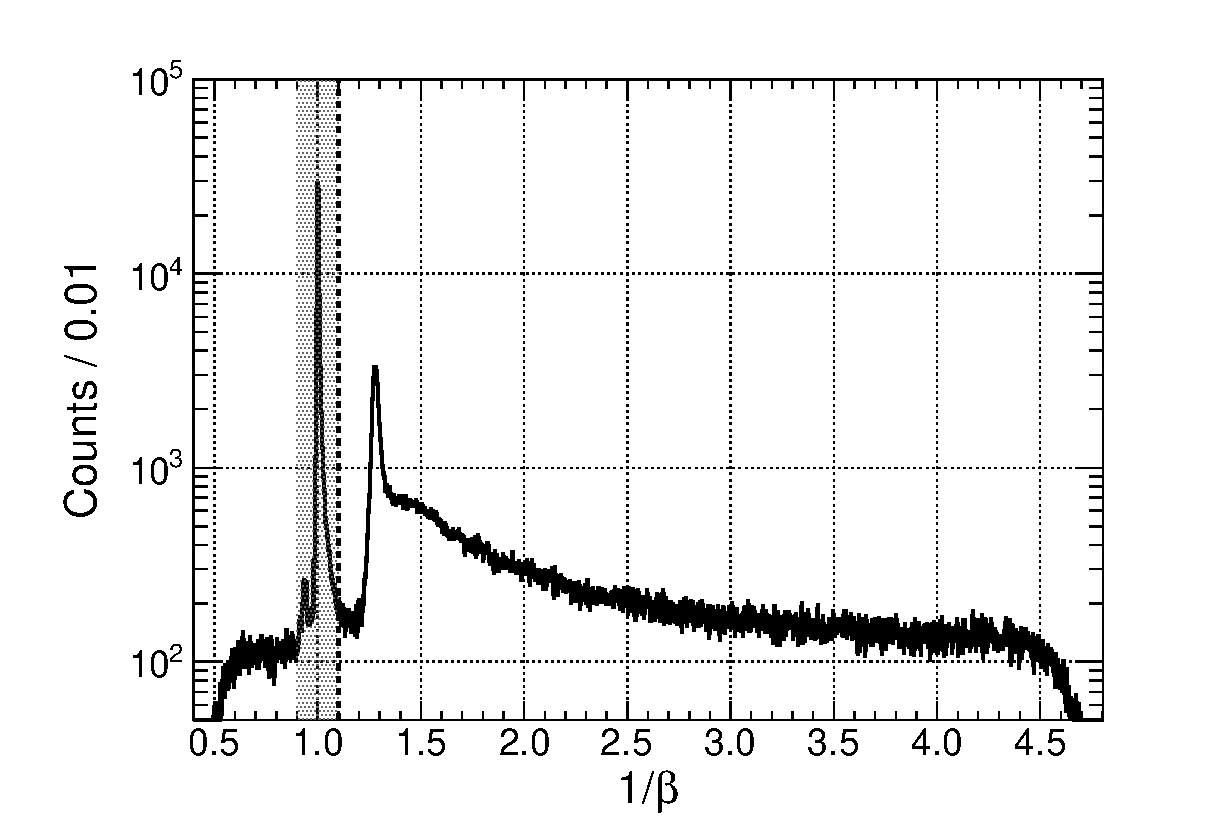
\includegraphics[width=12cm]{./fig/nc-beta.eps}
\caption[1/$\beta$ distribution of the forward neutral particles.]{1/$\beta$ distribution of the forward neutral particles detected with the NC. Right hand side of the dotted vertical line is identified as neutrons, while the hatched area represents the $\gamma$ selection. }
\label{fig-ncbeta}
\end{center}
\end{figure}  
 
\begin{figure}[]
\begin{center}
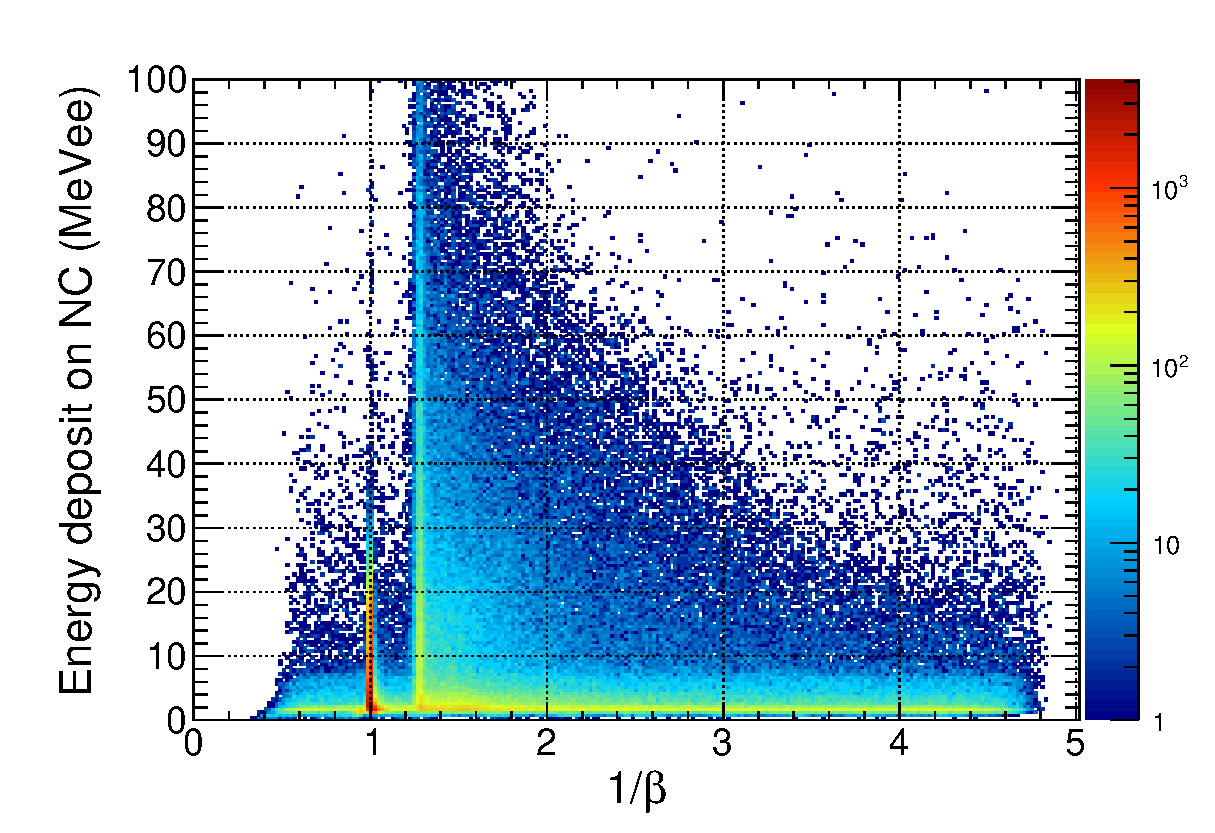
\includegraphics[width=12cm]{./fig/nc-betade.eps}
\caption{Distribution of the energy deposit on the NC and 1/$\beta$.}
\label{fig-ncbetade}
\end{center}
\end{figure}  

Figure \ref{fig-ncsn}(left) shows the $1/\beta$ distribution sliced in the various energy deposit regions. As naturally expected, the background contribution decreases with the higher energy deposit region. To quantitatively discuss this tendency, purity of the signal, $S/(S+B)$, is plotted as a function of energy deposit region in Fig. \ref{fig-ncsn}(right). Here we integrated the events in $1/\beta$=(1.15,1.35) as $S+B$ and the contribution of the accidental background $B$ was evaluated by fitting the spectrum in $1/\beta$=(0.6,0.9) with a constant function. We set the offline threshold to 8 MeV$ee$ where the purity almost saturates.

\begin{figure}[]
\begin{center}
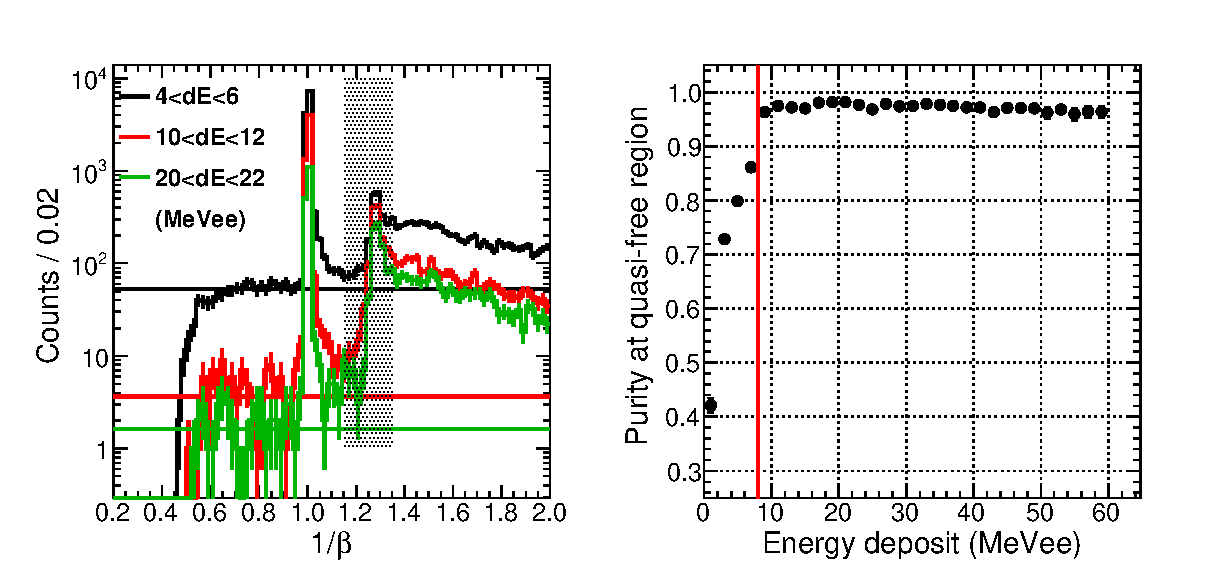
\includegraphics[width=\columnwidth]{./fig/nc-sn.eps}
\caption[Typical spectra with energy deposit slices and neutron purity dependence on the energy deposit.]{(left) Typical spectra with energy deposit slices. The horizontal lines shows the background level. Events in the hatched area were counted to derive the neutron purity. (right) Neutron purity dependence on the energy deposit. The offline analysis threshold was set to 8 MeV$ee$ as indicated with a red line.}
\label{fig-ncsn}
\end{center}
\end{figure}  


\subsection{Momentum resolution\label{sec-ncres}}
%\subsubsection{Threshold dependence}
%Another point is the resolution of neutron momentum. It is naturally expected that the resolution get better with a higher threshold. The resolution was evaluated by fitting $\gamma$-ray peak with a Gaussian. Figure \ref{} shows the threshold dependence of the $1/\beta$ resolution ($\sigma$) of the system.

\subsubsection{Momentum dependence}
The $1/\beta$ resolution of the neutral particle can be decomposed as,
\begin{eqnarray*}
\sigma_{\frac{1}{\beta}}\left(\frac{1}{\beta}\right) &=& \frac{1}{L_{vertex-NC}}\sqrt{\left(\frac{\sigma_z^{NC}}{\beta}\right)^2+\left(\left(\frac{1}{\beta}-\frac{1}{\beta_{beam}}\right)\cdot\sigma_z^{vertex}\right)^2+c^2\sigma_t^2}.
\end{eqnarray*}
The first term is a contribution from the uncertainty in the $z$ hit position of the NC. Assuming a uniform $z$ distribution of the hit position, $\sigma_z^{NC}=$5 cm/$\sqrt{12}$=1.44 cm is obtained. The second term is caused by the uncertainty of the $z$-vertex position. The $z$-vertex resolution was evaluated to be $\sigma_z^{vertex}$=0.7 cm in Sec. \ref{sec-cdsvres}. The last term comes from the intrinsic time resolution of T0 and the NC measured to be $\sim$110 ps with cosmic-ray data.

However, the measured $\gamma$-ray resolution cannot be reproduced by those values. Other effects such as the uncertainty in the $xy$ position, the neutral particles not from the reaction point, and the distortion of the flight length by scatterings might contribute. Here we made two independent assumptions to reproduce the resolution: additional deteriorations of $\sigma_t$ or $\sigma_z^{nC}$. The former has no $\beta$ dependence, namely the time measurement had worse resolution for some reasons, while the latter has the $\beta$ dependence which comes from the uncertainty in the flight length measurement. The data can be reproduced by deteriorating $\sigma_t$ from 110 ps to140 ps or $\sigma_z^{NC}\sim$ from 1.44 to 3 cm. The two cases were plotted in Fig. \ref{fig-ncresol} for the 1/$\beta$ and the neutron momentum resolutions. We adopted the mean of the two lines as the resolutions for the current analysis, and the deviation was considered as a systematic error. The neutron momentum resolution at $K^-pp$ binding threshold ($\sim$1.2 GeV/$c$) was evaluated to be 8.0$\pm$0.4 MeV/$c$.

\begin{figure}[]
\begin{center}
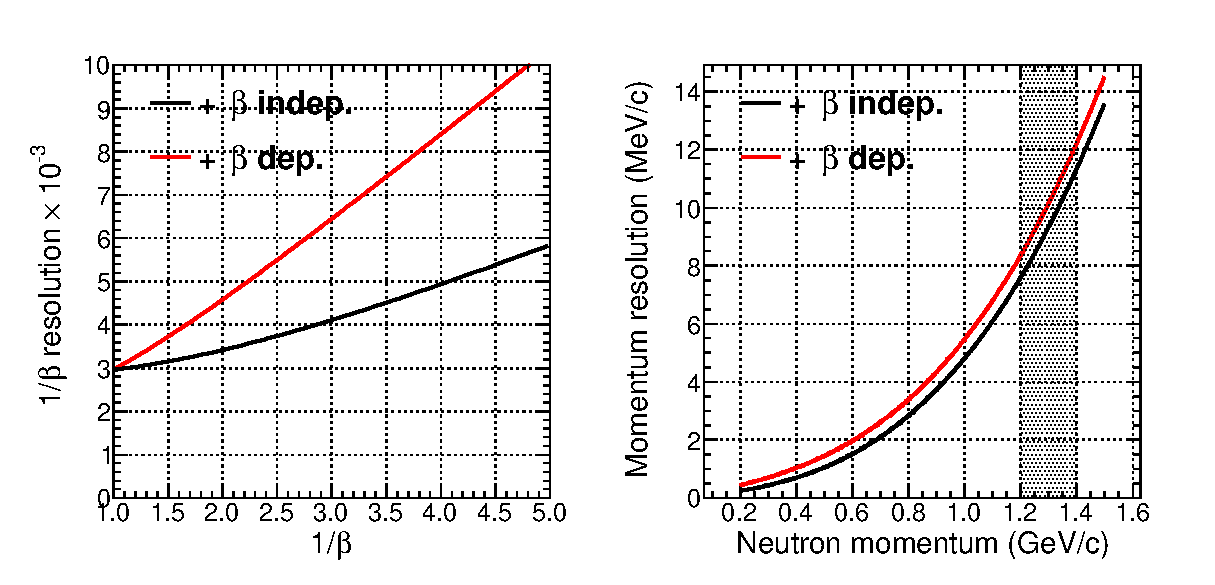
\includegraphics[width=\columnwidth]{./fig/nc-resol.eps}
\caption[Resolutions of the 1/beta and the neutron momentum.]{Resolutions of (left) the 1/beta and (right) the neutron momentum. The two curves correspond to the two independent assumptions in the resolution evaluation.}
\label{fig-ncresol}
\end{center}
\end{figure}  

\subsubsection{Stability and uniformity}
The $\gamma$-ray peak position and its resolution were stable during the experiment as shown in Fig. \ref{fig-ncrun}.  We also checked the uniformity of the 112 segments. % Figure \ref{} and Fig. \ref{} show the kaon-induced hit distributions of $\gamma$-rays and neutrons, respectively. The events has the continuous distributions.
Figure \ref{fig-ncseg} shows all the segment in the NC worked and calibrated fine.
\begin{figure}[]
\begin{center}
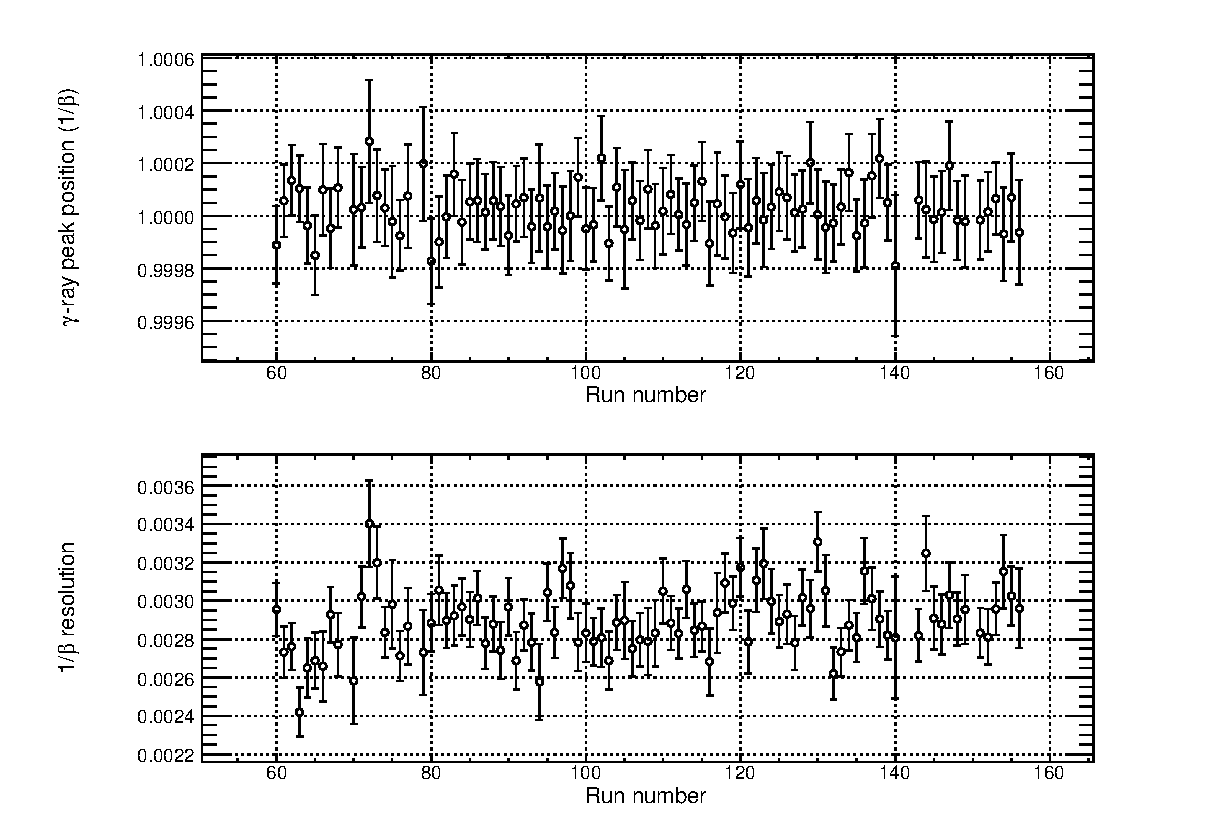
\includegraphics[width=\columnwidth]{./fig/nc-run.eps}
\caption[Run dependence of the $\gamma$-ray peak position and its resolution.]{Run dependence of (top) the $\gamma$-ray peak position and (bottom) its resolution.}
\label{fig-ncrun}
\end{center}
\end{figure}  
\begin{figure}[]
\begin{center}
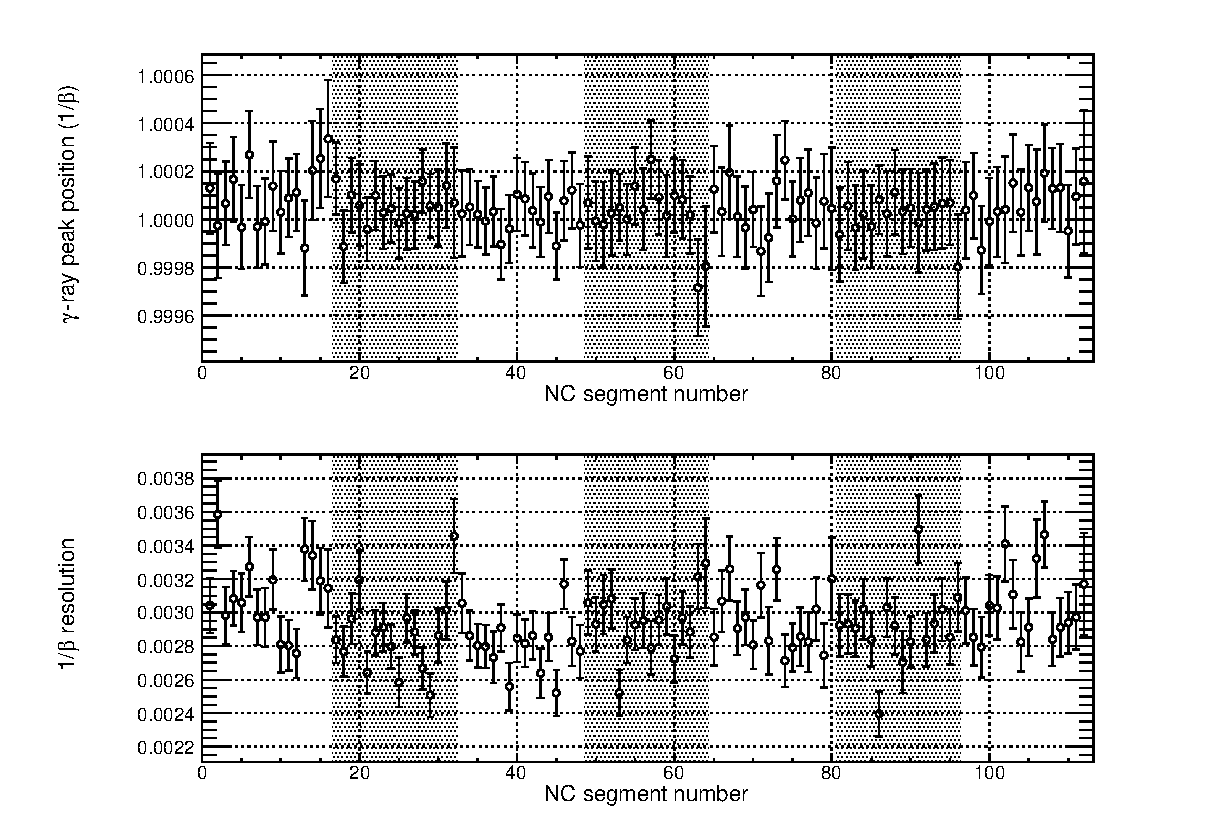
\includegraphics[width=\columnwidth]{./fig/nc-seg.eps}
\caption[NC segment dependence of the $\gamma$-ray peak position and its resolution.]{NC segment dependence of (top) the $\gamma$-ray peak position and (bottom) its resolution. The hatched areas represent the difference of the NC layers.}
\label{fig-ncseg}
\end{center}
\end{figure}  
